%*******************************************************************************
%****************************** Second Chapter *********************************
%*******************************************************************************

\ifpdf
\graphicspath{{Chapter2/Figs/}}
\else
\graphicspath{{Chapter2/Figs/}}
\fi

\chapter{Methods to Improve Privacy in Digital Currencies}
\label{ch:Methods to Improve Privacy in Digital Currencies}

The key to achieving anonymity in Bitcoin and any digital currencies is to remove the ability to link a payer to a payee. This immediately satisfies the third property of anonymity that it should be hard to link a payer to a payee. A user can also take advantage of this and make an anonymous payment to himself. Since the public key address that he uses to make the payment cannot be linked to the public key address that he uses to receive the payment, the user can transact with the latter public key address on a clean slate. Hence, the first and second properties of anonymity that it should be hard to link public key addresses and transactions to the same user are also achieved.

\section{Mixing}
\label{sec:2-Mixing}
Mixing is a concept that removes the ability to link a payer to a payee. All methods to improve privacy in digital currencies adopt mixing in one way or another by. The principle of mixing is illustrated in Fig.~\ref{fig:mixing}.

\begin{figure}[H]
	\begin{center}
		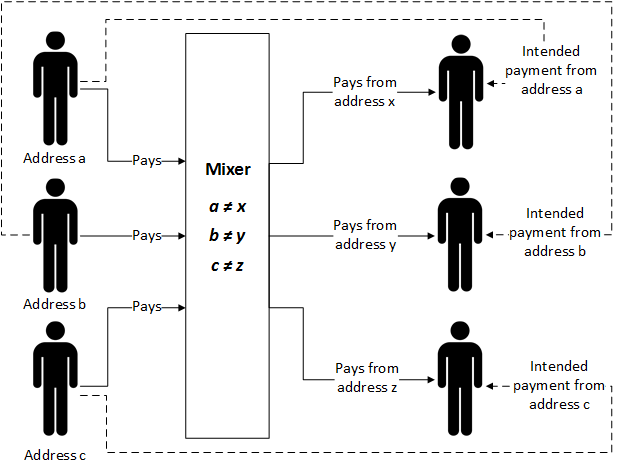
\includegraphics[scale=0.7]{mixing} 
		\caption{Principle of mixing}
		\label{fig:mixing} 
	\end{center}
\end{figure}

To perform mixing, payers make payments via an intermediary called the mixer. The mixer collects payments from payers and pays their intended payee via \kwTransaction{}{s} whose \kwInput{s} do not refer to the public key address of the original payers. In this way observers of the Blockchain are only able to see \kwTransaction{}{s}  from the payers to the mixer and from the mixer to the payee, but cannot tell which payer paid to which payee. The anonymity set in this case is the number of payers participating in the mix, since one only knows that a payer participated in the mixing, but is unable to tell who the payer paid to among the payees that received payments from the mixer.

In order for mixing to work, the amounts that is being transacted via a mixer should be constant for all participants of the mixing protocol \cite{narayanan2016bitcoin}. If different payers pay different amounts to the mixer, and subsequently the mixer pays different amounts to the payees, one can deduce the link between a payer and payee by matching the payment amounts between the payer and the mixer and those between the mixer and the payee. This research has explored several methods of mixing and the issues they face. 

\section{Dedicated Mixing Services and Decentralised Mixing}
\label{sec:2-Dedicated Mixing Services and Decentralised Mixing}
\textbf{Dedicated mixing services} have been commercially implemented in Bitcoin. Services such as Bitcoin Fog and BitLaundry routinely handle 6-digit dollar amounts everyday \cite{Moser2013}. These services act as centralised mixers, where participants make payments to the services and instruct them to transfer the funds to specific address. However dedicated mixing services face some major drawbacks:

\begin{enumerate}
	\item Dedicated mixing services need to keep the transactions records of their users to make fund transfers. Thus privacy is built on the trust that mixing services will not disclose these records. This runs against decentralized principle of Bitcoin and digital currencies in general \cite{narayanan2016bitcoin}.
	\item Since mixers are used for payments, users typically require funds to be transferred immediately to the intended payees. Thus mixers can only work with a limited pool of participants who happen to make payments at the same time. This limits the anonymity set in the mixing protocol, and lowers the level of anonymity in the protocol \cite{narayanan2016bitcoin}.
	\item By exploiting the weakness in point 2 and analysing the mixing patterns adopted by the dedicated mixers, transactions in dedicated mixes can be de-anonymised \cite{Moser2013}. 
\end{enumerate}

\textbf{Decentralised mixing} adopts a peer-to-peer mixing protocol. One such protocol proposed is Coinjoin \cite{Gmaxwell2013}, which gathers payers who wish to participate in mixing to collectively construct a single transaction. Each \kwInput{} in the Coinjoin transaction refers to the funds from each payer, while each \kwOutput{} in the transaction pays to the public key address of each intended payee. The \kwInput{s} and \kwOutput{s} are ordered randomly in the transaction, and an adversary cannot tell which input (payer) corresponds to which output (payee). Here the mixer is the transaction, and the anonymity set is the number of participants in the transaction. Though Coinjoin achieves decentralisation, it still faces the same problem as dedicated mixing services of having a limited anonymity set, as the protocol is carried out with the few payers who want to make payments at the same time. In addition, since a Conjoin transaction is collectively constructed, the protocol faces denial-of-service attacks where an adversary who initially agrees to participate in a Coinjoin transaction refuses to complete his part in the creation of the transaction \cite{narayanan2016bitcoin}.

As seen, Bitcoin mixing techniques that involve the shuffling to payers and payees do not work well in both the centralised and decentralised form. There is also little room for improvement for these protocols as any bigger changes will involve modifications to the Bitcoin protocol that are too costly to implement. Altcoins, on the other hand, have the liberty implement any protocol and thus provide a higher level of anonymity compared to the mixing protocols.

\section{Altcoins: Zerocoin and Zerocash}
\label{sec:2-Altcoins: Zerocoin and Zerocash}
Altcoins are alternative digital currency systems to Bitcoin. The two popular proposed altcoins that provide privacy are Zerocoin and Zerocash. As opposed to the traditional mixers discussed in \S\ref{sec:2-Dedicated Mixing Services and Decentralised Mixing}, Zerocoin and Zerocash provides anonymity using cryptographic guarantees. As these two protocols are very technical, they are only dealt with in concept, with a focus on their capabilities and drawbacks and the reasons why Zerocoin is chosen as the final subject of research. The Zerocoin protocol will then be examined in detail in \S\ref{ch:Analysis of Zerocoin}. Unless otherwise stated, all technical information presented on Zerocoin and Zerocash are obtained from the original Zerocoin \cite{Miers2013} and Zerocash \cite{Ben-Sasson2014} papers.

\subsection{Zerocoin}
\subsubsection{Protocol}
\label{sec:2-Zerocoin Protocol}
Zerocoin extends Bitcoin by incorporating another type of anonymous currency called the “Zerocoin” into the Bitcoin protocol. A comparison between Bitcoin and Zerocoin is shown in Fig.~\ref{fig:zerocoin_overview}.

\begin{figure}[H]
	\begin{center}
		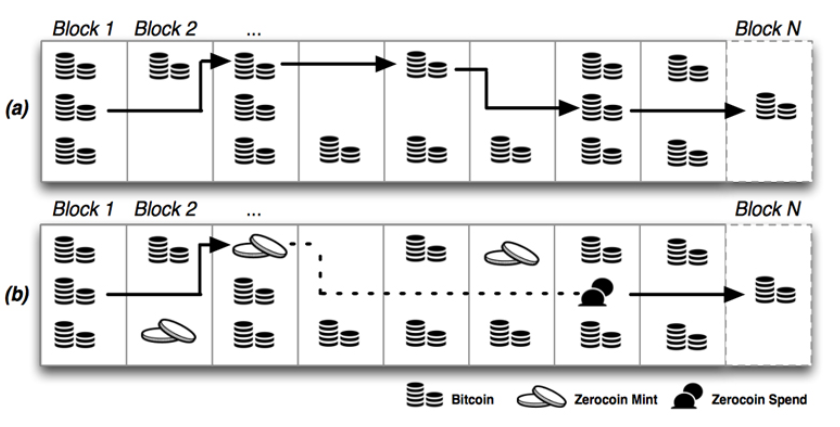
\includegraphics[scale=0.7]{zerocoin-overview} 
		\caption{Comparison between Bitcoin and Zerocoin \cite{Miers2013}}
		\label{fig:zerocoin_overview} 
	\end{center}
\end{figure}

Payments in Bitcoin (a) involves a transfer of funds (Bitcoins) via \kwTransaction{}{s} recorded on the Blockchain. In any block, payments are made using Bitcoins that have been paid to the payer in a previous block (i.e. transaction \kwInput{s} refer to \kwOutput{s} of past \kwTransaction{}{s}).
 
The high level flow of Zerocoin (b) is also similar. In addition to using Bitcoins for payments, users can use their Bitcoins to create an anonymous “Zerocoin” (referred to as \kwCoin{} from now on) via a \kwTransaction{Mint }{}. The exchange rate between Bitcoin and \kwCoin{} is fixed, and thus a Bitcoin always mints the same amount of \kwCoin{}. A \kwCoin{} is a cryptographic commitment $c$ of a serial number $S$ and a secret trapdoor $r$ which are only known to the user who minted the \kwCoin{}. The property of $c$ is that both $S$ and $r$ is needed to obtain the value of $c$, and it is hard to compute the value of $S$ or $r$ from $c$. Like a Bitcoin \kwTransaction{}{}, a \kwTransaction{Mint }{} contains \kwInput{s} that specify the Bitcoins that are used to mint the \kwCoin{}. A \kwTransaction{Mint }{} does not have an \kwOutput{} as it does not make any payment and simply creates a \kwCoin{}. Once the \kwInput{} in a \kwTransaction{Mint }{} is verified to be valid by nodes, it is published on the Blockchain and the minted \kwCoin{} $c$ is added to a public data structure called the \textbf{accumulator} (\S\ref{sec:3-Public Accumulator}). 

The minted \kwCoin{} $c$ can be redeemed and converted to back to Bitcoins later on using a \kwTransaction{Spend }{}. Similar to a Bitcoin \kwTransaction{}{}, the \kwTransaction{Spend }{} contains an \kwInput{} that proves the ownership of $c$, and an \kwOutput{} that specifies the public key address to pay the converted Bitcoins to. To prove of ownership of $c$ in the \kwTransaction{Spend }{}, the redeemer must prove:

\begin{enumerate}
	\item The knowledge of the serial number $S$ and random trapdoor $r$ that produced $c$ (\S\ref{sec:3-Serial Number Signature of Knowledge})
	\item $c$ has been previously minted and added to the accumulator (\S\ref{sec:3-Accumulator Proof of Knowledge})
\end{enumerate}


To prove the above, the \kwTransaction{Spend }{} only reveals $S$ that is committed in the redeemed $c$ and $c$ itself is not revealed. Such proofs are called Non-Interactive Zero Knowledge (NIZK) proof which are discussed in detail in \S\ref{sec:3-NIZK Proofs in Zerocoin}. Once the proof is verified the \kwTransaction{Spend }{} gets published on the Blockchain and the \kwOutput{} in the transaction can be subsequently referred to and spent by its owner. To prevent the redeemed $c$ from being redeemed again, $S$ is disclosed and recorded on a separate public table. Any \kwTransaction{Spend }{s} that spends a \kwCoin{} with a serial number that is listed on the  will be rejected. A simplified example illustrating the links between normal Bitcoin \kwTransaction{}{s}, \kwTransaction{Mint }{s} and \kwTransaction{Spend }{s} is shown in Fig.~\ref{fig:zerocoin_transactions}.

\begin{figure}[H]
	\begin{center}
		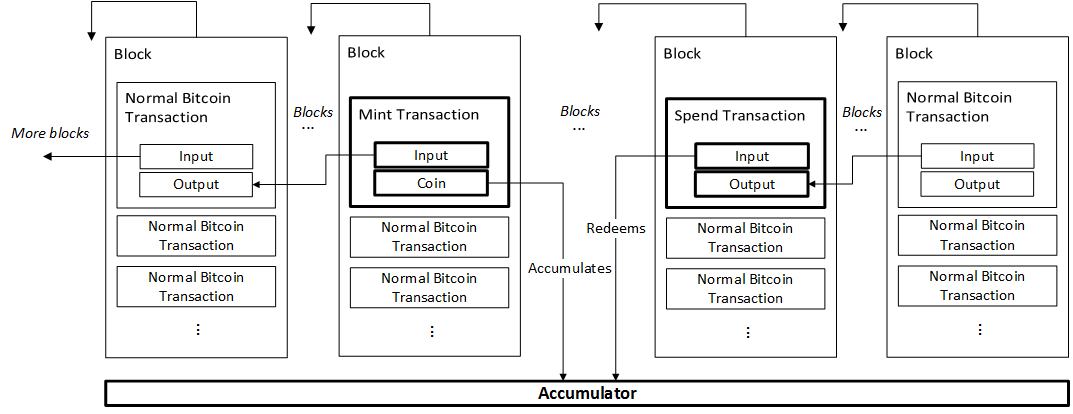
\includegraphics[scale=0.525]{zerocoin-transactions} 
		\caption{Links between Bitcoin \kwTransaction{}{s}, \kwTransaction{Mint }{s} and \kwTransaction{Spend }{s}}
		\label{fig:zerocoin_transactions} 
	\end{center}
\end{figure}

Zerocoin is in fact a mixing protocol, where minted \kwCoin{s} act as the intermediary. When a new \kwTransaction{Mint }{s} is published on the Blockchain, the minted \kwCoin{} $c$ is mixed with the rest of the previously minted \kwCoin{s} in the Accumulator. When a \kwTransaction{Spend }{} is published on the on the Blockchain, the only information available to the public is that one of all the previously minted \kwCoin{s} has been redeemed to a public key address as the redeemed \kwCoin{} is not revealed. Even though the serial number $S$ of the redeemed \kwCoin{} is revealed to verify that it has not been spent, the secret trapdoor $r$ is private to the \kwCoin{}’s owner at all times. An adversary who only know $S$ cannot determine which $c$ is being redeemed and thus cannot link the redeemer of the Zerocoin (payee) to the user who minted this \kwCoin{} (payer). Hence the anonymity set in Zerocoin is all of the minted and unredeemed \kwCoin{s} in history, which is much larger than the anonymity sets in the traditional Bitcoin mixing protocols (\S\ref{sec:2-Dedicated Mixing Services and Decentralised Mixing}). Therefore Zerocoin achieves a much higher level of anonymity compared to these protocols.

\subsubsection{Drawbacks}
\label{sec:2-Zerocoin Drawbacks}
However Zerocoin is not a perfect system. Some of the drawbacks of Zerocoin are listed below:

\begin{enumerate}
	\item \kwCoin{s} can only have fixed denominations, making payments less flexible. The reason behind the fixed denominations is to ensure that adversaries find it hard to match transaction amounts between Mint and \kwTransaction{Spend }{s} to determine links between them. This is largely similar to why transaction amounts in traditional mixing protocol must be uniform for all participants (\S\ref{sec:2-Dedicated Mixing Services and Decentralised Mixing}). 
	\item There is no provision to transfer a \kwCoin{} to a payee directly, and actual payments still need to be done in Bitcoins. Every time a payer wants to make a payment, he needs to redeem a \kwCoin{} to Bitcoins via a \kwTransaction{Spend }{}, and make the payment using the Bitcoins via a normal Bitcoin \kwTransaction{}{}. If the payee wants to make an anonymous payment again using the received Bitcoins, he must first mint some \kwCoin{s} via a \kwTransaction{Mint }{} and then redeem them via a \kwTransaction{Spend }{}. Thus \kwCoin{s} need to be constantly minted and redeemed to cater for multiple anonymous transactions. This makes anonymising transactions using Zerocoin cumbersome. 
	\item The payment amounts, payment addresses and the timings of Zerocoin transactions are still publicly available on the Blockchain. This means that Zerocoin is still exposed to side channel attacks (\S\ref{sec:1-Side Channels Attacks}).
	\item Zerocoin \kwTransaction{Spend }{s} are much larger in size (50KB) compared to Bitcoin \kwTransaction{}{s} (1KB) due to the large size of the NIZK proofs that are used to prove the ownership of \kwCoin{s}. This is undesirable in a peer-to-peer digital currency network. Firstly, since all nodes in the network maintains a copy of the Blockchain, large transactions sizes increase the storage requirement of nodes. Secondly, large transactions also take longer time to be propagated in the peer-to-peer network, which slows down the confirmation of transactions and the overall performance of the system.
\end{enumerate}

\subsection{Zerocash}
\subsubsection{Protocol}
\label{sec:2-Zerocash Protocol}
Zerocash is purported to be an improvement of Zerocoin. It is built on the same principles as Zerocoin, where a \kwTransaction{Mint }{} create some \kwCoin{s} and a Pour transaction (Similar to \kwTransaction{Spend }{} in Zerocoin) spends a minted \kwCoin{} without disclosing which \kwCoin{} is spent. Instead of using the NIZK proofs in Zerocoin to prove ownership of \kwCoin{s}, Zerocash does this by using zero-knowledge Succinct Non-interactive Arguments of Knowledge (zk-SNARKs) \cite{Ben-sasson2013}. As zk-SNARKs is extremely complex and a relatively new field, this research is not able to describe how the proof works. However its features is sufficient to evaluate Zerocash as a protocol. The improvements in Zerocash from Zerocoin that are made possible by zk-SNARKs are listed below:

\begin{enumerate}
	\item The size of the proofs for the ownership of \kwCoin{s} in Zerocash is reduced from 45KB to 288B. As such Zerocash transactions have similar size as the standard Bitcoin \kwTransaction{}{s} (1KB). 
	\item The time taken to verify a \kwTransaction{Pour }{} in Zerocash is reduce by 98.6%.
	\item Zerocash transactions hide all transaction details. The only information that is publicly available in a transactions are the zk-SNARKs proofs to verify the transactions. Hence one can only observe the existence of a transaction on the Blockchain and other information such as transaction amounts and payment addresses are hidden. This makes side channel attacks (\S\ref{sec:1-Side Channels Attacks}) impossible.
	\item Zerocash supports arbitrary denominations since the transaction amounts are hidden and cannot be exploited by side channel attacks.
	\item Zerocash allows minted \kwCoin{s} to be directly transferred from payer to payee. There is no need to redeem a \kwCoin{} into Bitcoins before payments can be made like in Zerocoin.
\end{enumerate}

\subsubsection{Drawbacks}
\label{sec:2-Zerocash Drawbacks}

Though seemingly superior, Zerocash also has the following weaknesses when compared to Zerocoin:

\begin{enumerate}
	\item The theoretical foundation of Zerocash has not be proven to be sound. zk-SNARKs is a relatively new area of research and its theories have not been used in practice as of 2015 \cite{narayanan2016bitcoin}. In contrast, the NIZK proofs used by Zerocoin, which are based on RSA cryptography (\S\ref{sec:3-Non-Interactive Zero Knowledge (NIZK) Proofs}), has been widely tested and proven for many years. 
	\item Zerocash requires a huge set of parameters (over 1GB) for the zk-SNARKs proofs. This places a huge storage constraint for anyone who wishes to use Zerocash, and makes deployment of Zerocash on mobile devices challenging. In contrast, Zerocoin only requires a single parameter of about 2.5KB for its NIZK proofs.
	\item The construction of the zk-SNARKs proofs in Zerocash computationally expensive. Specifically, it takes 2 minutes to construct the proofs in a \kwTransaction{Pour }{} using an Intel Core i7 3.40GHz processor with 16GB of RAM. This means that a user of Zerocash needs to wait for 2 minutes before he/she can create a transaction on a high-end PC. This makes Zerocash impractical for mobile devices with lower processing power. In contrast, on a machine that has similar processing power as the above mentioned Intel Core i7 processor, Zerocoin only requires 0.7s to construct a \kwTransaction{Spend }{}.
\end{enumerate}

\subsection{Selection Zerocoin as the Subject of Research}
\label{sec:2-Selection Zerocoin as the Subject of Research}
A summary of the key features of Zerocoin and Zerocash is listed in Table~\ref{tab:zerocash_zerocoin_keyfeatures}.

\begin{table}[H]
	\centering \small
	\begin{tabular}{ p{5.5cm} | p{4.25cm} | p{4.25cm} }
		
		& \textbf{Zerocoin} & \textbf{Zerocash} \\ 		
		\hline
		\hline
		\textbf{Technology} & 
		RSA cryptography. Mature and proven in practice. & 
		zk-SNARKs. New and not implemented in practice. \\	
		\hline
		\textbf{Level of anonymity} & Payment amount, timing and addresses are public. Susceptible to side channel attack. & Only transaction timing is public, hides all other transaction information. Side channel attack is not possible. \\
		\hline
		\textbf{Denomination} & Fixed & Arbitrary \\ 
		\hline
		\textbf{Direct payment using \kwCoin{s}} & No & Yes \\
		\hline
		\textbf{Size of parameters} & 2.5KB & 1GB \\	
		\hline
		\textbf{Size of proof} & 45KB & 288B \\
		\hline
		\textbf{Time taken to construct the proofs in a \textit{Spend/Pour transaction }on a high end processor} & 2 minutes & 0.7s \\
		\hline
		\textbf{Time taken to verify the proofs in a \textit{Spend/Pour transaction} on a high end processor} & 300ms & 5.7ms \\
		
	\end{tabular}
	\caption{Key features of Zerocoin and Zerocash}
	\label{tab:zerocash_zerocoin_keyfeatures}
\end{table}


Zerocash definitely has much more to offer in terms of privacy and features. However Zerocash requires large storage and a long time to construct transactions even on high-end processors, and thus may face challenges running on clients that increasingly consist of mobile devices. Though the transaction sizes of Zerocoin are relatively large and may impose higher load on the peer-to-peer network, the overall storage and processing requirements of Zerocoin for both the clients and the network is still moderate. Slight improvements in Zerocoin’s performance can make it a very practical protocol. 

In addition, the technology behind Zerocash is also not mature. Literature on zk-SNARKs is both sparse and complex, while literature on NIZK proofs are readily available and well documented \cite{Zcoin2016}. This makes research on Zerocoin more productive compared to Zerocash. Moreover the theoretical basis for Zerocash is uncertain due to the lack of implementation of zk-SNARKs in real-life applications, while Zerocoin is theoretically reliable as it uses NIZK proofs which are tested and proven. 

Most importantly, the full anonymity provided by Zerocash may be undesirable. This is because full anonymity removes a key feature of the Blockchain, which is that the peer-to-peer network can collectively audit the public transactions. If payment amounts in transactions are hidden, any bugs or attacks that cause \kwCoin{s} to be wrongly created will go unnoticed on the Blockchain. This can cause hyperinflation of Zerocash and render the system obsolete \cite{Zcoin2016}. Thus as promising as it seems, Zerocash has its caveats and its implications as a real-life digital currency system are unknown. 

Taking into account the above considerations, Zerocoin is a more attractive area of research due to its performance, the accessibility of literature and its potential application. Hence the rest of this research devotes to analysing Zerocoin in detail and finding ways to improve its performance, so that it can be a practical anonymous digital currency system. 
